\documentclass[11pt]{article}

\usepackage{geometry}
 \geometry{
 a4paper,
% total={210mm,297mm}
% }
 left=17mm,
 right=23mm,
 top=20mm, 
 bottom=20mm,
}

\bibliographystyle{apalike}
\usepackage{url}
\usepackage{rotating}
\usepackage{natbib}
\usepackage{placeins}
\usepackage{longtable}
\usepackage[latin1]{inputenc}
\usepackage{multirow}
\usepackage{hyperref}
%\usepackage{showframe}
\usepackage{pdflscape}
%\usepackage{pbox}
\usepackage{xcolor}
\usepackage{amsmath}
\usepackage{rotating}
\usepackage{multicol}
\usepackage{caption}
\usepackage{subcaption}
\usepackage{xspace} % see http://tex.stackexchange.com/questions/31091/space-after-latex-commands


\usepackage{pdflscape}

\usepackage{listings}

\lstset{
  basicstyle=\ttfamily, 
  basewidth=0.5em,                 %the default setting of listings with "fixed columns" has a space 0.6em wide, 
                                   %while the characters in Computer Modern Typewriter are 0.5em wide.
                                   %http://tex.stackexchange.com/questions/179071/spacing-looks-wrong-in-listings-when-using-fixed-columns
  backgroundcolor=\color{gray!10},
  keywordstyle=\color{green!40!black},
  columns=fixed,
  language=R,                     % the language of the code
  basicstyle=\footnotesize,       % the size of the fonts that are used for the code
  numbers=left,                   % where to put the line-numbers
  numberstyle=\tiny\color{gray},  % the style that is used for the line-numbers
  stepnumber=1,                   % the step between two line-numbers. If it's 1, each line
                                  % will be numbered
  numbersep=5pt,                  % how far the line-numbers are from the code
  showspaces=false,               % show spaces adding particular underscores
  showstringspaces=false,         % underline spaces within strings
  showtabs=false,                 % show tabs within strings adding particular underscores
  frame=single,                   % adds a frame around the code
  rulecolor=\color{black},        % if not set, the frame-color may be changed on line-breaks within not-black text (e.g. commens (green here))
  tabsize=2,                      % sets default tabsize to 2 spaces
  captionpos=b,                   % sets the caption-position to bottom
  breaklines=true,                % sets automatic line breaking
  breakatwhitespace=false,        % sets if automatic breaks should only happen at whitespace
  title=\lstname,                 % show the filename of files included with \lstinputlisting;
                                  % also try caption instead of title
  keywordstyle=\color{blue},      % keyword style
  commentstyle=\color{green},   % comment style
  stringstyle=\color{red},      % string literal style
  escapeinside={\%*}{*)},         % if you want to add a comment within your code
  morekeywords={*,...}            % if you want to add more keywords to the set
} 

\usepackage{graphicx}
\usepackage{gensymb}
\usepackage{nag}   %It warns the user about the usage of old packages or commands (for example, using \it, \tt, etc.)
\usepackage{fixltx2e}
%fixltx2e package. It fixes some 'mistakes' in Latex. From the description:
%        ensure one-column floats don't get ahead of two-column floats;
%        correct page headers in twocolumn documents;
%        stop spaces disappearing in moving arguments;
%        allowing \fnysmbol to use text symbols;
%        allow the first word after a float to hyphenate;
%        \emph can produce caps/small caps text;
\usepackage{booktabs}
% \centering instead of \begin{center} \end{center} to center things inside tables/figures etc. \centering doesn't add any additional vertical space.
\usepackage{microtype}  %for small-scale typographic enhancements (character protrusion, font expansion, letter-spacing).
\usepackage{fancyvrb}   %get precise control in verbatim listings.
%\usepackage{siunitx} To typeset units
\usepackage{numprint} %format numbers nicely 
%~, the non-breakable space.

\parindent=0pt
\parskip=8pt
\setlength\itemsep{0em}

%\sloppy
%\SweaveOpts{echo=FALSE,prefix.string=script18/plot}
\renewcommand{\textfraction}{0.0}

\let\oldmarginpar\marginpar
\renewcommand\marginpar[1]{\-\oldmarginpar[\raggedleft\footnotesize #1]%
{\raggedright\footnotesize #1}}

\newcommand{\supp}{\mathop{\mathrm{supp}}}


\usepackage{xspace} % 
%\usepackage{showframe}

\newcommand{\cursedforest}{\textsc{CursedForest}\xspace}
\newcommand{\ranger}{\textsc{Ranger}\xspace}
\newcommand{\randomforest}{\textsc{randomForest}\xspace}
\newcommand{\mtry}{\texttt{mtry}\xspace}
\newcommand{\ntree}{\texttt{ntree}\xspace}

\newsavebox\ltmcbox

\title{The Donoho-Tanner Phase Transition}
\author{}
\date{}



\begin{document}
%\setkeys{Gin}{width=8cm}
\setkeys{Gin}{height=8cm,width=0.9\columnwidth}
\maketitle
%%\tableofcontents
%% ## \begin{landscape}
%% ##   \small
%% ## \end{landscape}


%% \begin{lstlisting}
%% \end{lstlisting}


\section{Introduction}
We consider the question of variable recovery in a sparse linear system, $y=X \beta + \epsilon,$ where only
a small number, $k$, of the $\beta$ variables are not equal to 0. We would like the solution,
\[
\min_\beta \rVert \beta \rVert_0 \textrm{ s.t. } y = X\beta,
\]
however; this is computationally infeasible for larger numbers of variables. We have to approximate the solution by
minimizing some $l_1$ or $l_2$ criteria, or by a more limited heuristic search of the solution space.
\cite{Donoho.and.Tanner.2009} and \cite{Donoho.and.Stodden.2006}  have considered this problem and introduce a ``phase
diagram'' to help explore the behaviour of various approaches.
This is implemented in the Matlab library \url{https://sparselab.stanford.edu}.

My aims in this exercise have been threefold:
\begin{itemize}
\item to investigate these ideas  in R. To this end I have replicated the example and some of the plots from
  \cite{Donoho.and.Stodden.2006};
\item to see if a ranking method like rank-biased-overlap (RBO) \cite[]{Webber2010} will allow us to extend some of these
  ideas to methods that do not produce an estimate of the $\beta$ coefficients. See section \ref{section:the.Rank.biased.Overlap.measure} for a brief
  discussion of RBO;
\item to see how a random forest behaves on the simulation used in \cite{Donoho.and.Stodden.2006}.
\end{itemize}

\section{The phase transition}
\cite{Donoho.and.Tanner.2009} give a ``universal phase change'' result that has applications in a
large number of areas, including variable selection in high dimensions.

The phase change boundary is
shown in Fig~\ref{figure:phase-diagram-equivalence.png} in the ``phase space'' parameterized by the level of underdetermination,
$\delta = n/p$, and by the sparsity, $\rho =k/n$ (where $k$ is the number of informative variables).  
They argue that there is a sharp disjunction between the cases where informative variables may be recovered with a high
accuracy by procedures like stepwise variable selection, and the cases where they can not be recovered. Above the
phase-transition line variable recovery is still possible by an exaustive search.

The theoretical phase change boundary is based on arguments from combinatorial geometry.

\begin{figure}[tbhp] 
    \centering
    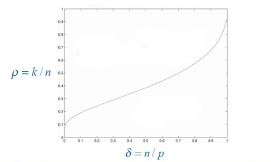
\includegraphics[totalheight=6cm,width=12cm]{./figs/phase2.png} %-diagram-equivalence.png} 
    \caption{The phase change diagram. Below the line informative variables may be recovered with a high
      accuracy. Above the line a combinatorial search is required. Reproduced from \protect{\cite{Donoho.and.Stodden.2006}}.}
    \label{figure:phase-diagram-equivalence.png} 
    \vspace{4ex}
\end{figure}

\FloatBarrier
\section{A simulation}
\cite{Donoho.and.Stodden.2006} investigate the phase transition in a small simulation.  They consider a regression
problem with $\underset{n\times p}{X}\sim N(0,1)$ with $p$ fixed at 200 and $n$ variable. Figures \ref{figure:k.png} and
\ref{figure:n.png} show the phase space colored by $n$ and $k.$

\begin{figure}[tbhp] 
    \begin{subfigure} [b]{0.5\linewidth}
      \centering
      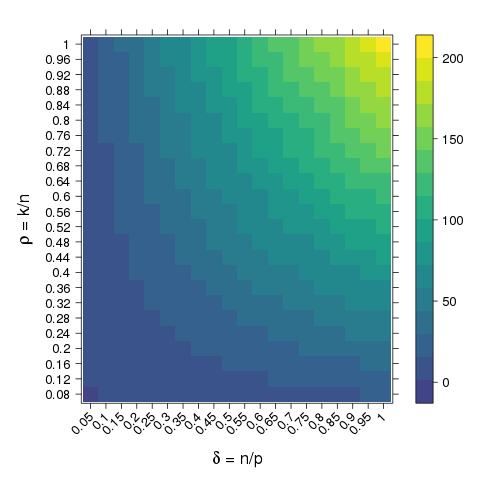
\includegraphics[totalheight=6cm]{./figs/k.png}
      \caption{$k$}
      \label{figure:k.png}
    \end{subfigure} 
    \begin{subfigure}[b]{0.5\linewidth}
      \centering
      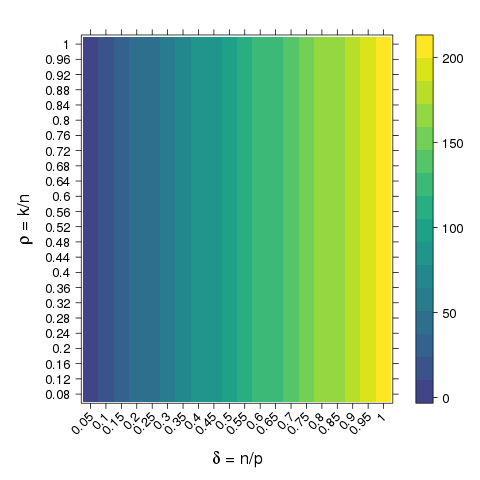
\includegraphics[totalheight=6cm]{./figs/n.png}
      \caption{$n$}
      \label{figure:n.png}
    \end{subfigure} 
    \caption{The simulation in \protect{\cite{Donoho.and.Stodden.2006}} considers $\delta = n/p$ and $\rho =k/n$. Here we plot the
      space of $\{\delta, \rho$\}, colored  by the paramters $n$ and $k.$}
\end{figure}

They set $\beta(1:k) \sim U(1,100)$ and $\beta((k+1):p) =0$, then $y= X\beta + \epsilon$ with
$\epsilon \sim N(0,\sqrt{16})$. They evaluate variable selection by the normalized $l_2$ error measure
$$\frac{\Vert\hat{\beta}-\beta\Vert_2}{\Vert\beta\Vert_2}.$$

They consider a number of variable selection methods, including a false discovery rate criteria. This involves adding
the variable with the maximum $t$-value to the linear model if the $p$-value is less than
$0.25(\text{number of terms currently in the model})/(\text{total number of variables})$.  See
Fig~\ref{figure:error_Stodden_FDR.png} for the error measure and figure \ref{figure:rbo_Stodden_FDR.png} for the RBO,
comparing the ranking (i.e. values) of $\hat{\beta}$ and $\beta$. It apparent that the accuracy of the  error measure
shows a marked drop in line with the prediction of the Donoho-Tanner phase transition. The behaviour of the RBO measure
is less clear.

Figure \ref{figure:transect.png} shows the error values for $\delta=0.5$ in for the data from Figure
\ref{figure:error_Stodden_FDR.png}. The sudden nature of the change can be seen.


\begin{figure}[tbhp] 
  \begin{subfigure}[t]{0.5\linewidth}
    \centering
    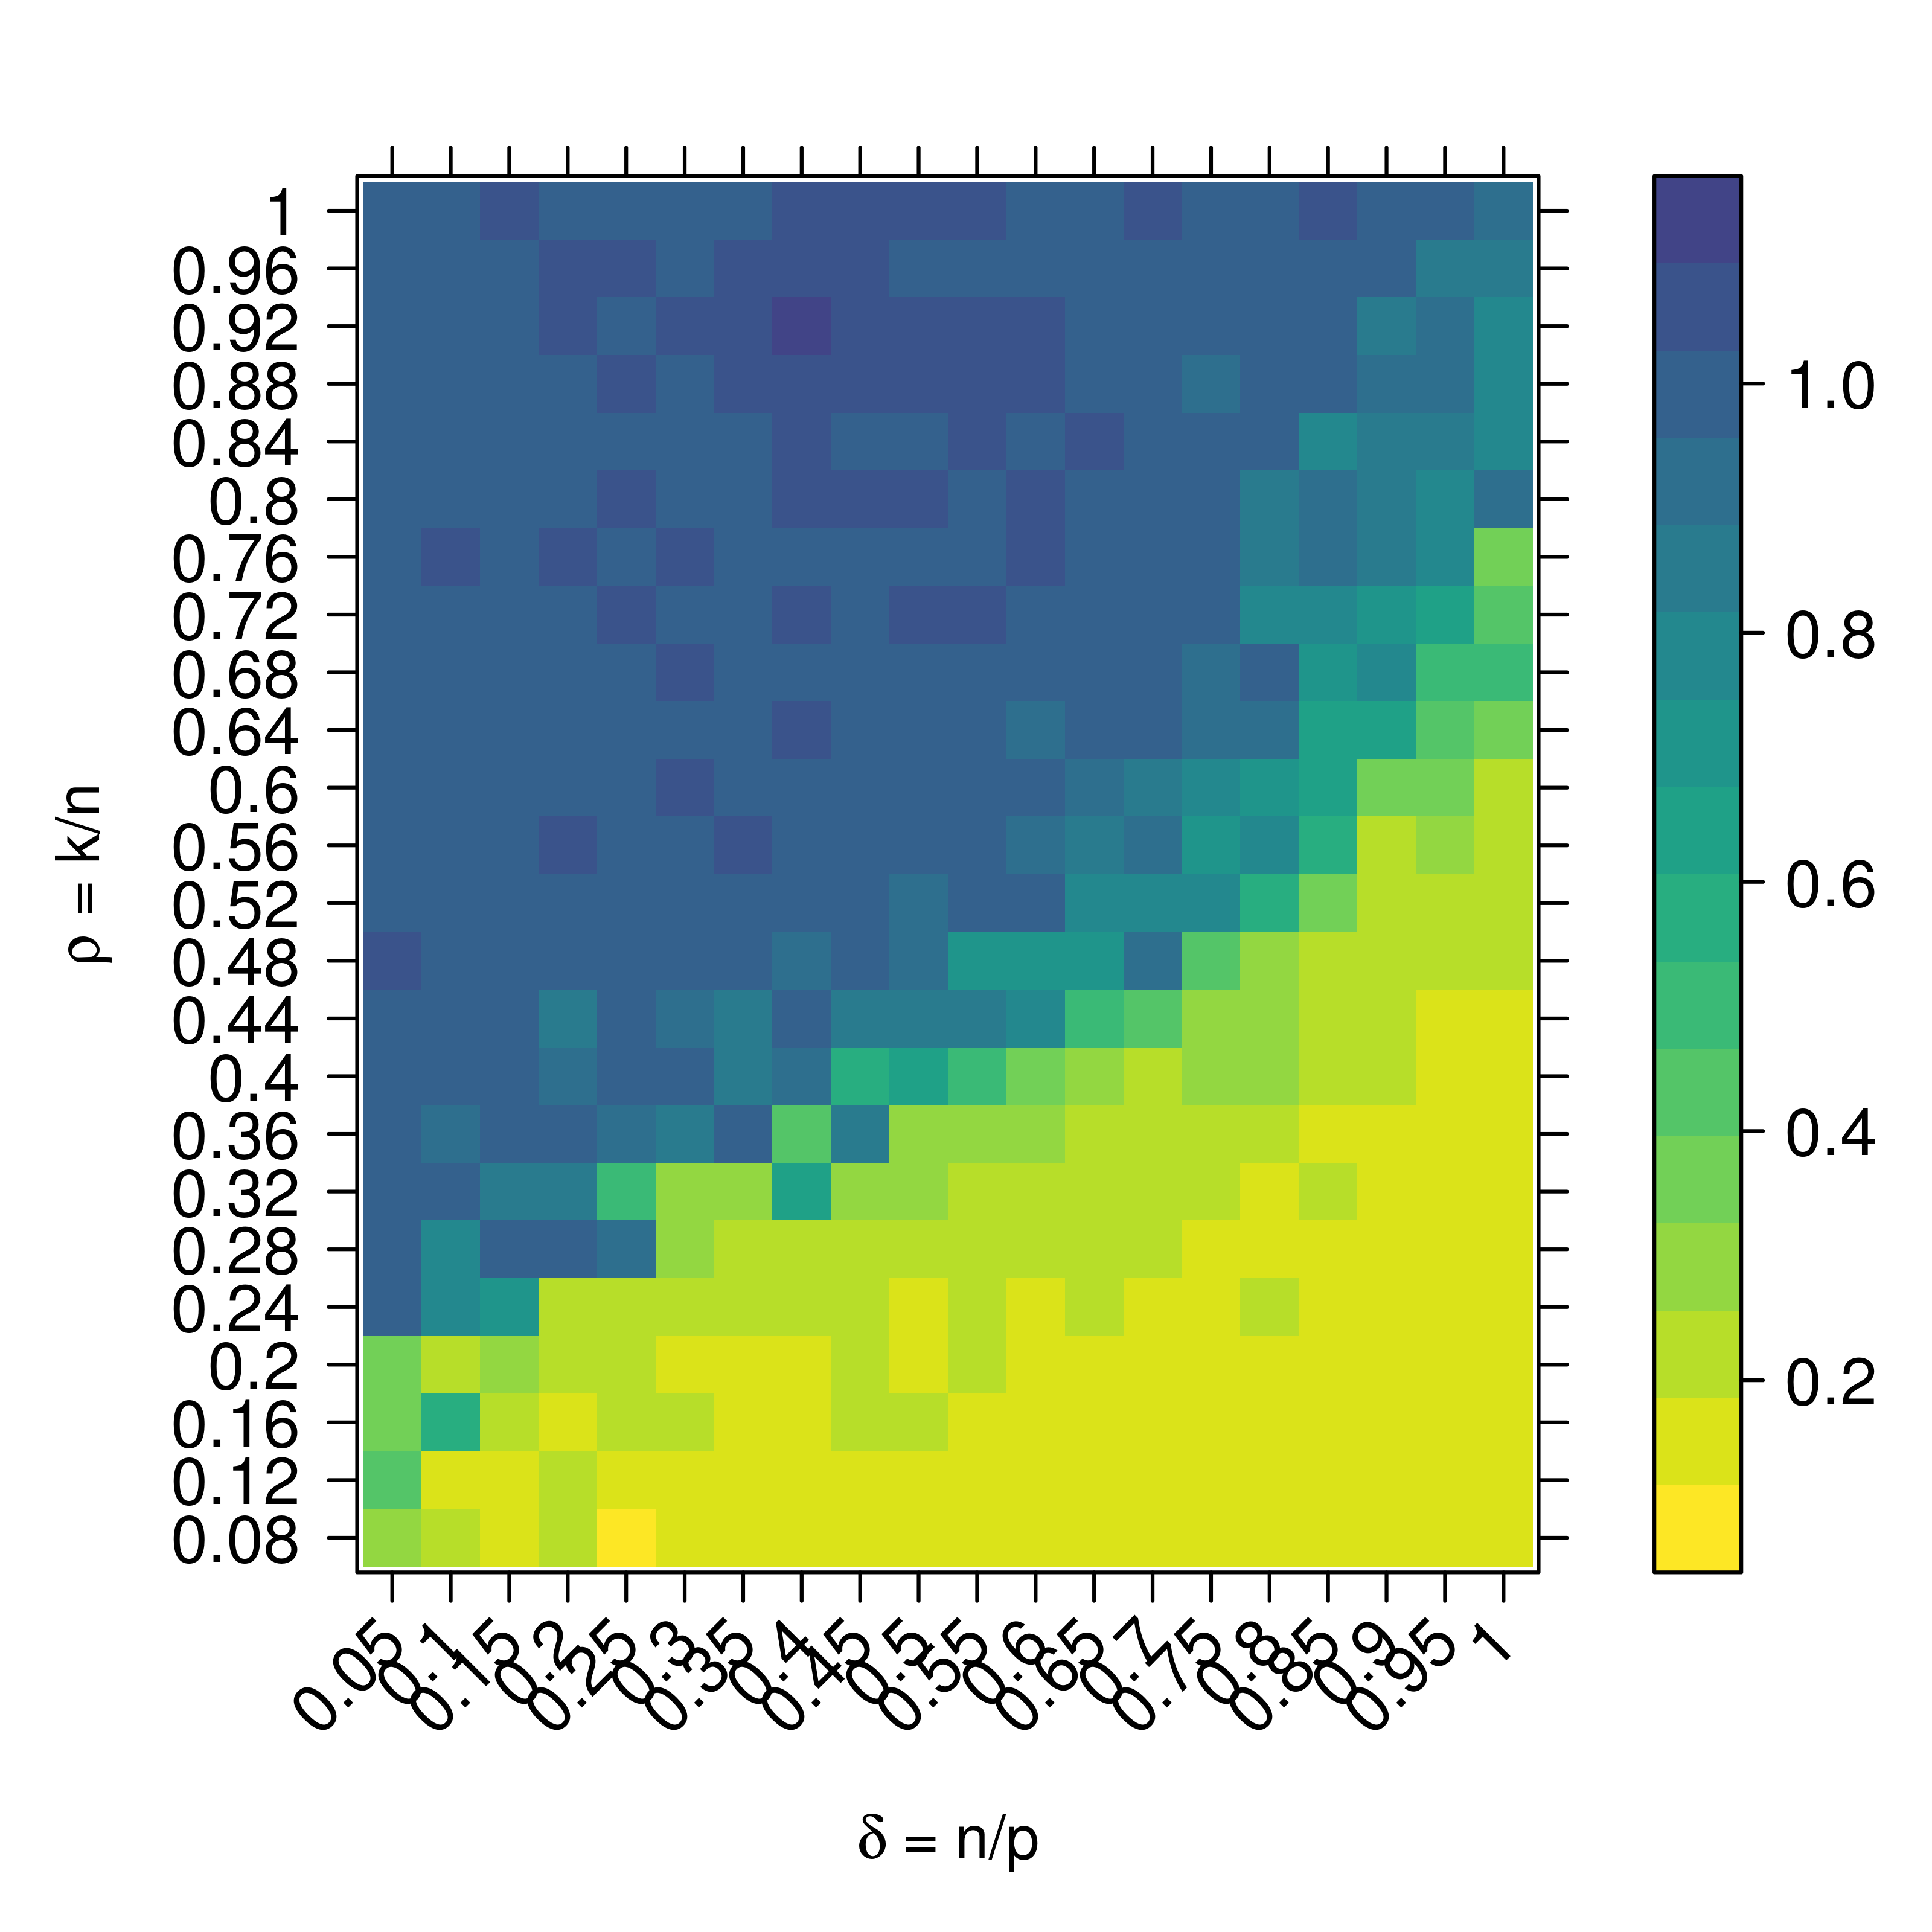
\includegraphics[totalheight=6cm]{./figs/error_Stodden_FDR.png}
    \caption{The error measure.}
    \label{figure:error_Stodden_FDR.png}
  \end{subfigure} 
  \begin{subfigure}[t]{0.5\linewidth}
    \centering
    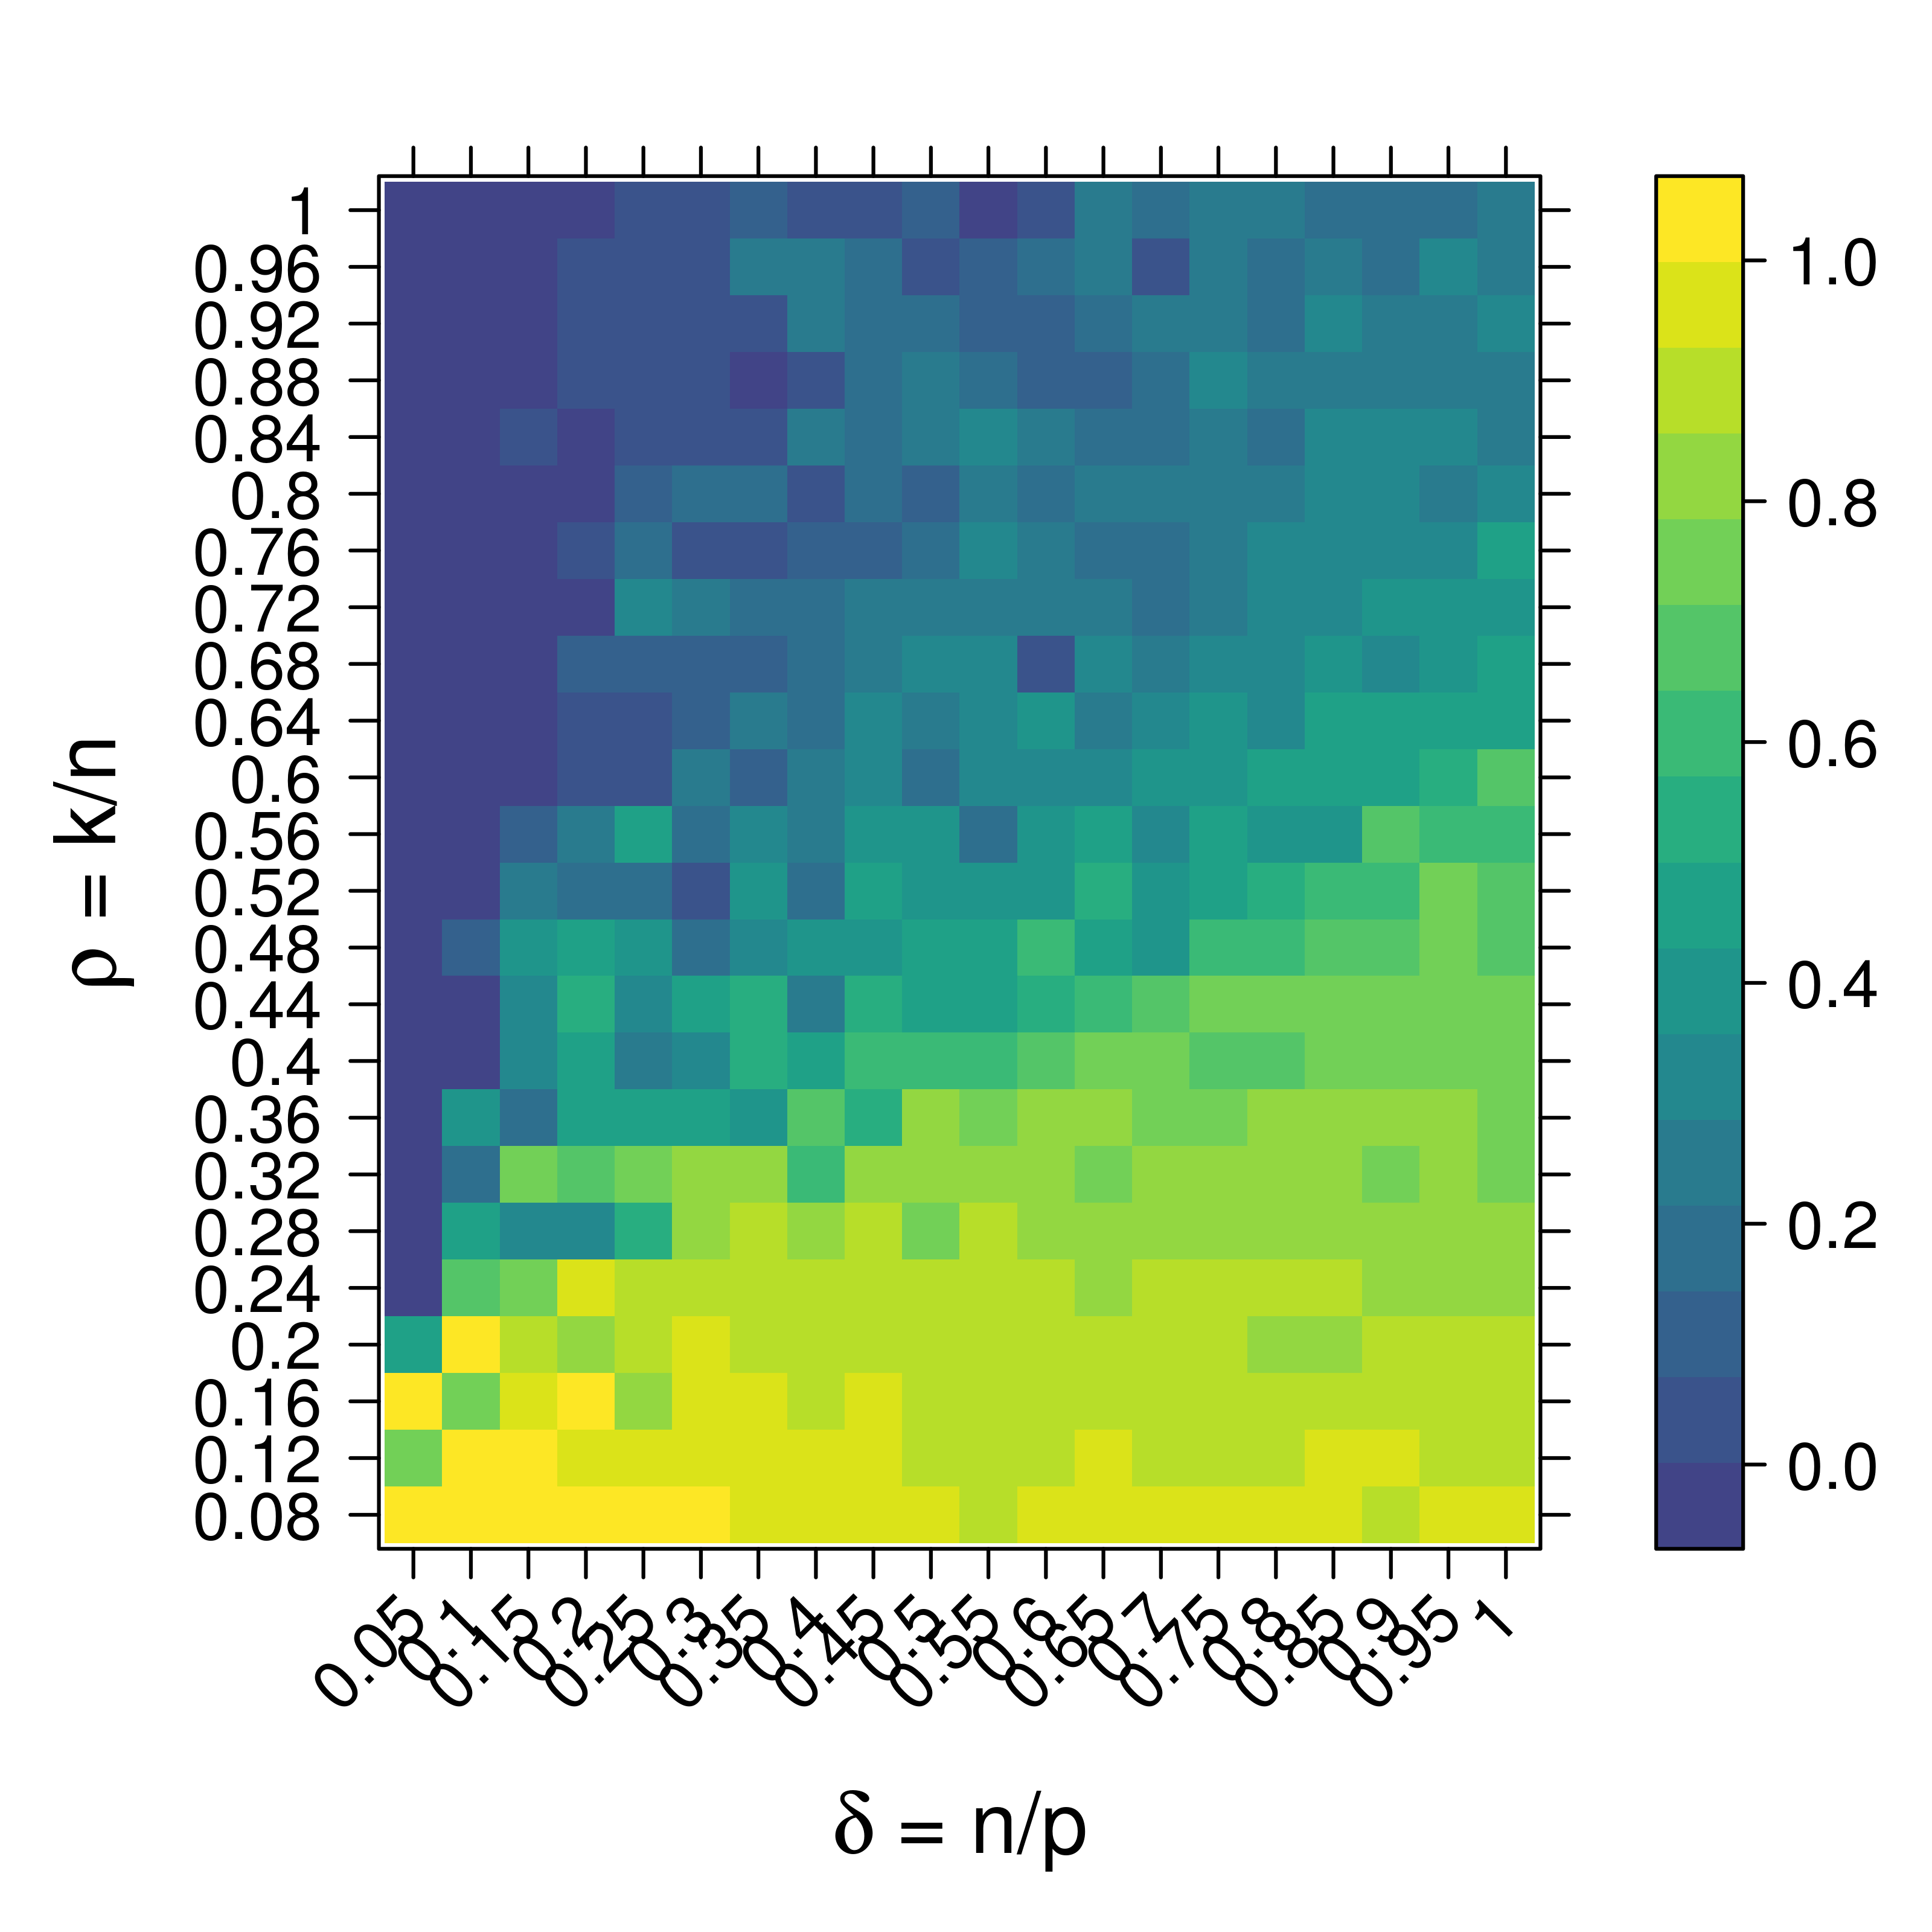
\includegraphics[totalheight=6cm]{./figs/rbo_Stodden_FDR.png}
    \caption{The RBO measure}
    \label{figure:rbo_Stodden_FDR.png}
  \end{subfigure} 
  \caption{Forward stepwise variable selection with a false discovery
    rate stopping criteria. Note that the plot colors have been chosen so that the lighter color indicates
      the better result, that is, a lower error or a higher RBO.}
  \label{figure:error_and_rbo_Stodden_FDR.png}
\end{figure}


\section{Random Forests on the simulated data}
% We have seen no work on the question of such a phase transition in the case of classification problems. Still it may be
% instructive to consider the implications of the pahse transition for our work. As \cursedforest is designed for
% extremely large numbers of variables it is likely to be operating in difficult regions of the figure where the ratio
% $\delta = n/p$ is small. In the simulated example in section \ref{***} the underdeterminedness $\delta = 0.002$ and the
% sparsity $\rho =2\times 10^{-6}$

We have used a random forest (the \ranger package, see \cite{Wright.and.Ziegle.2016})
on the same data as used for Fig~\ref{figure:error_and_rbo_Stodden_FDR.png}. The
Donoho-Tanner phase transition arises in recovering the $\beta$ in data generated by a linear model. However, in a
decision tree (random forest) we are fitting a non-linear model and there is no notion of estimating the
$\beta$. Becsaue of this we have evaluted the performance of the random forest using the RBO measure
on the variable importance.

We note that while a random forest is a long way from an all-subsets search, it is a limited search of the feature
space. As such it may perform outside of the bounds of the phase transition. 

Fig~\ref{figure:ranger_error_and_rbo_Stodden_simulation.png} shows the OOB prediction error and the RBO error for a
random forest with 10000 trees and the \mtry value set to the default for a regression problem (depending on $n$). It
shows no evidence of following the shape of the Donoho-Tanner phase transition.

\begin{figure}[tbhp] 
  \begin{subfigure}[t]{0.5\linewidth}
    \centering
    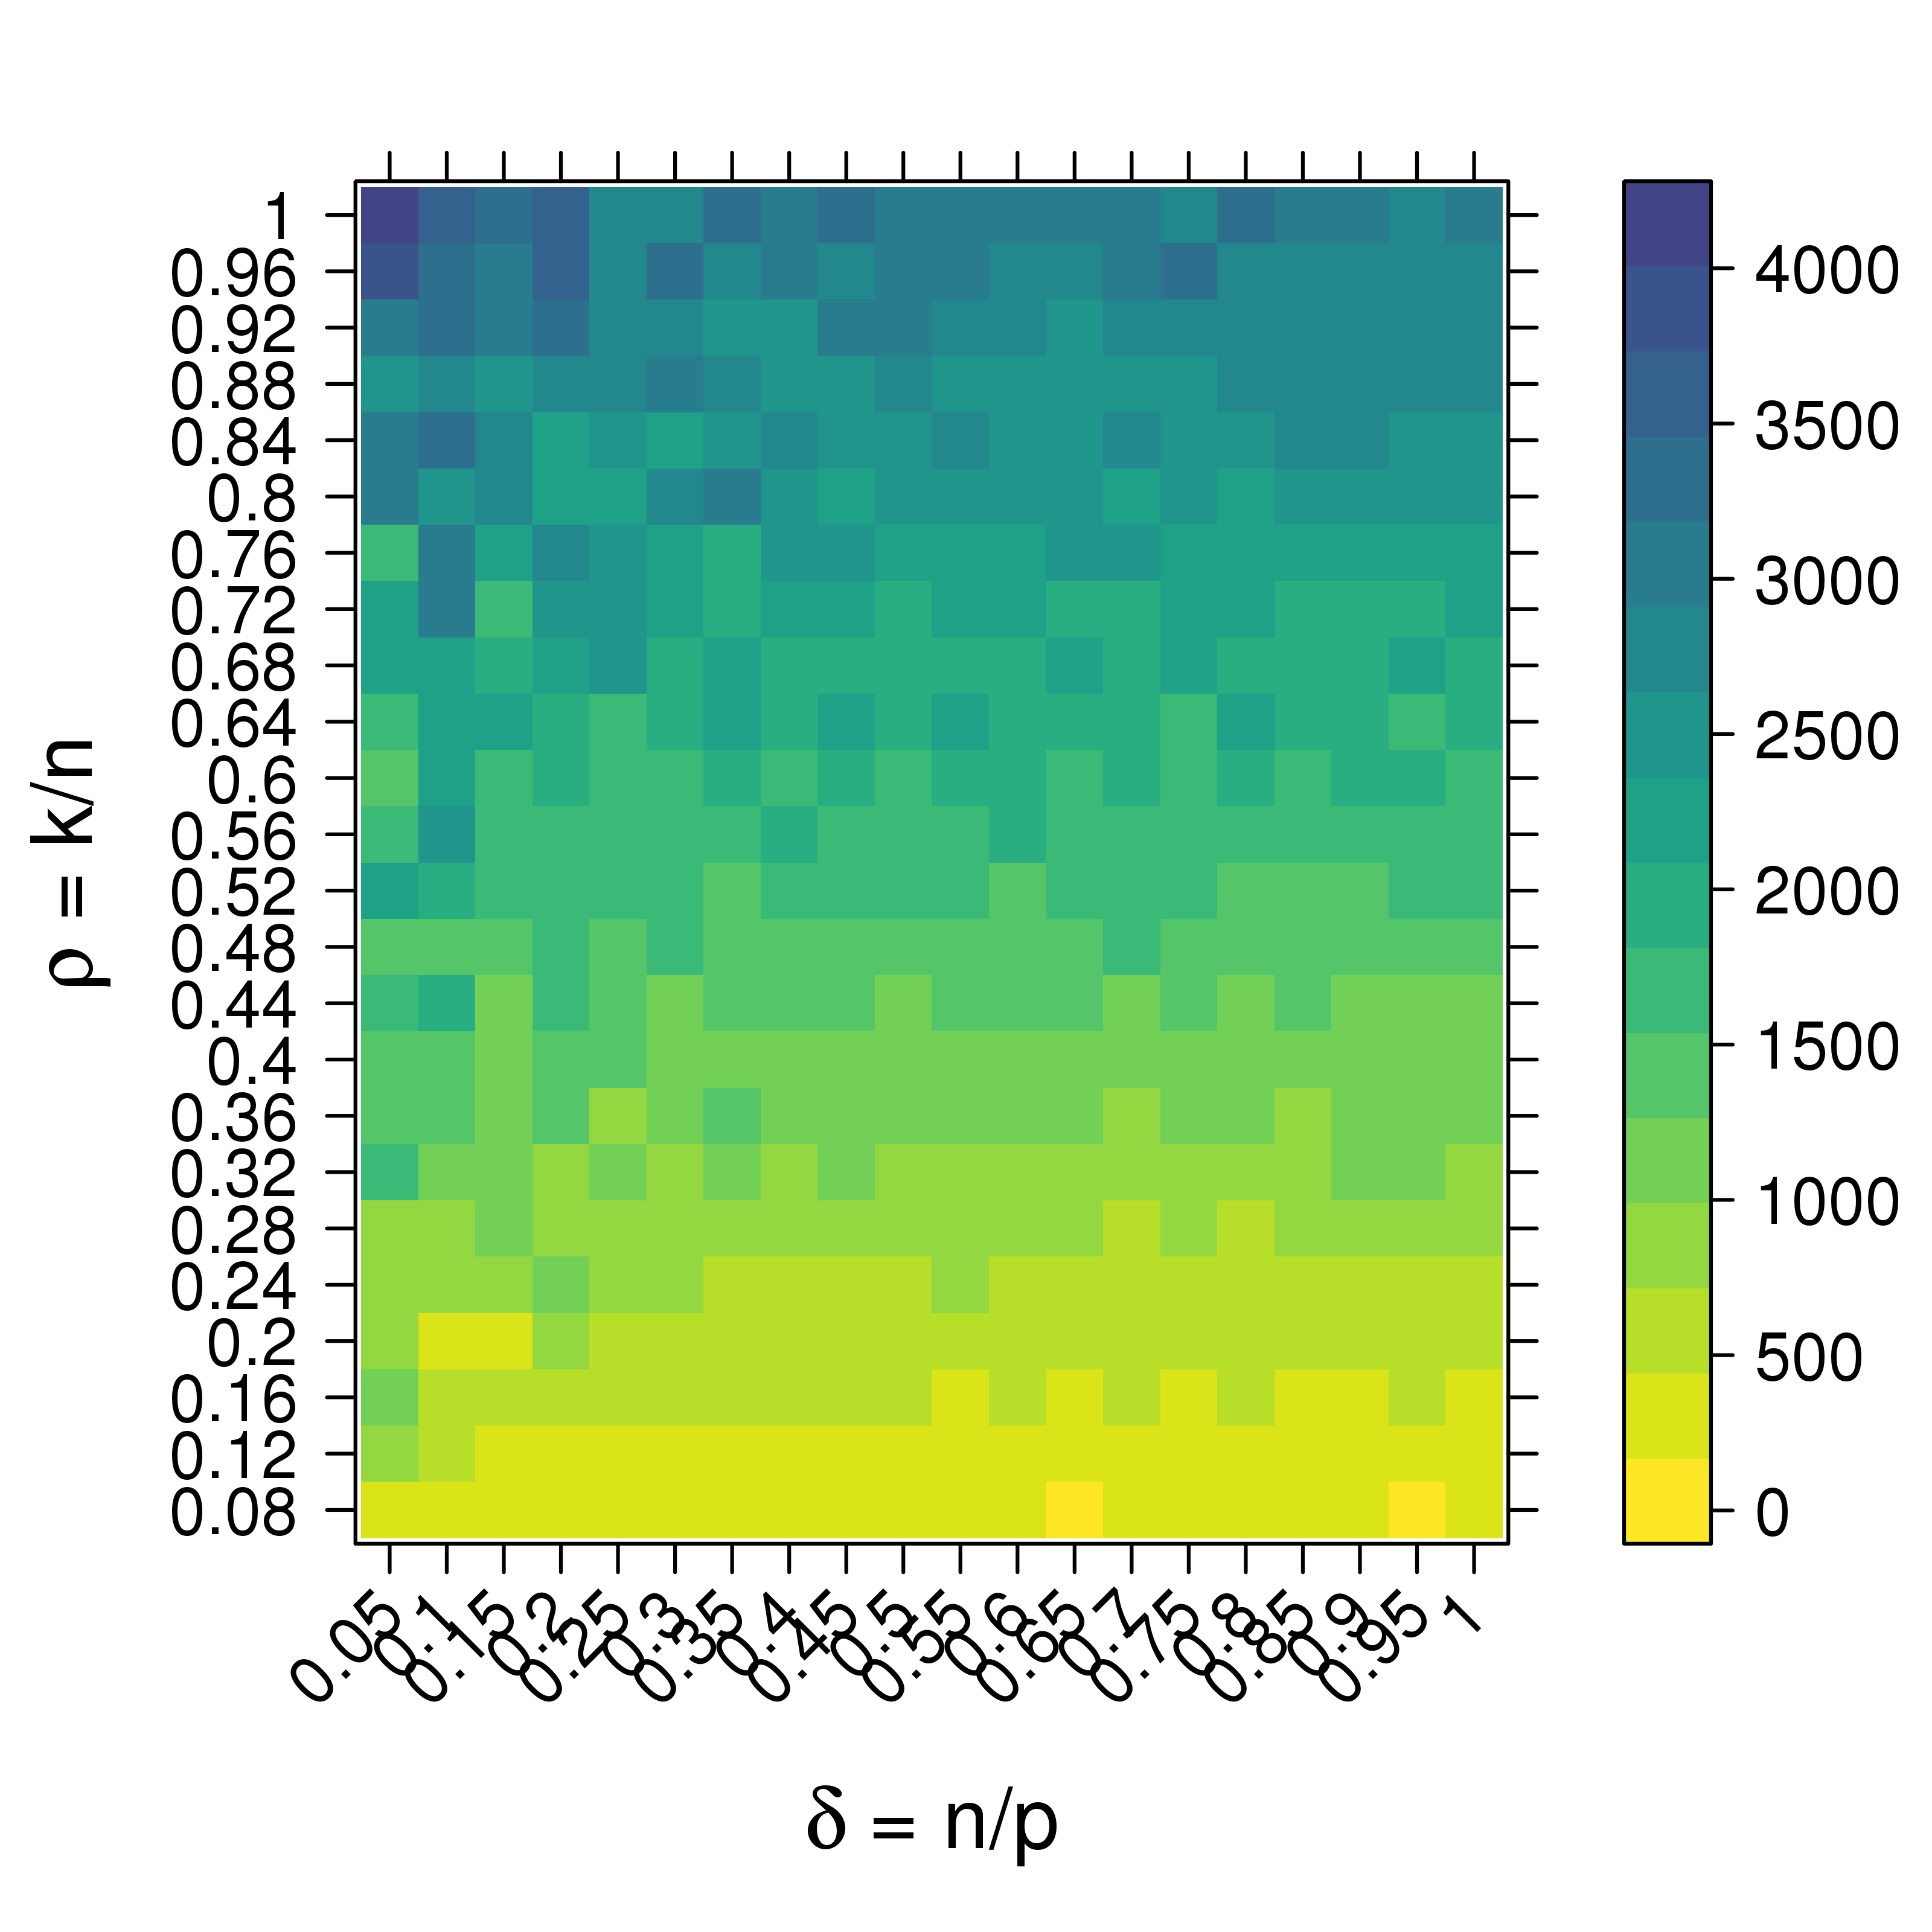
\includegraphics[totalheight=6cm]{./figs/ranger_error_Stodden_simulation.png}
    \caption{The out-of-bag error.}
    \label{figure:ranger_error_Stodden_simulation.png}
    \vspace{4ex}
  \end{subfigure} 
  \begin{subfigure}[t]{0.5\linewidth}
    \centering
    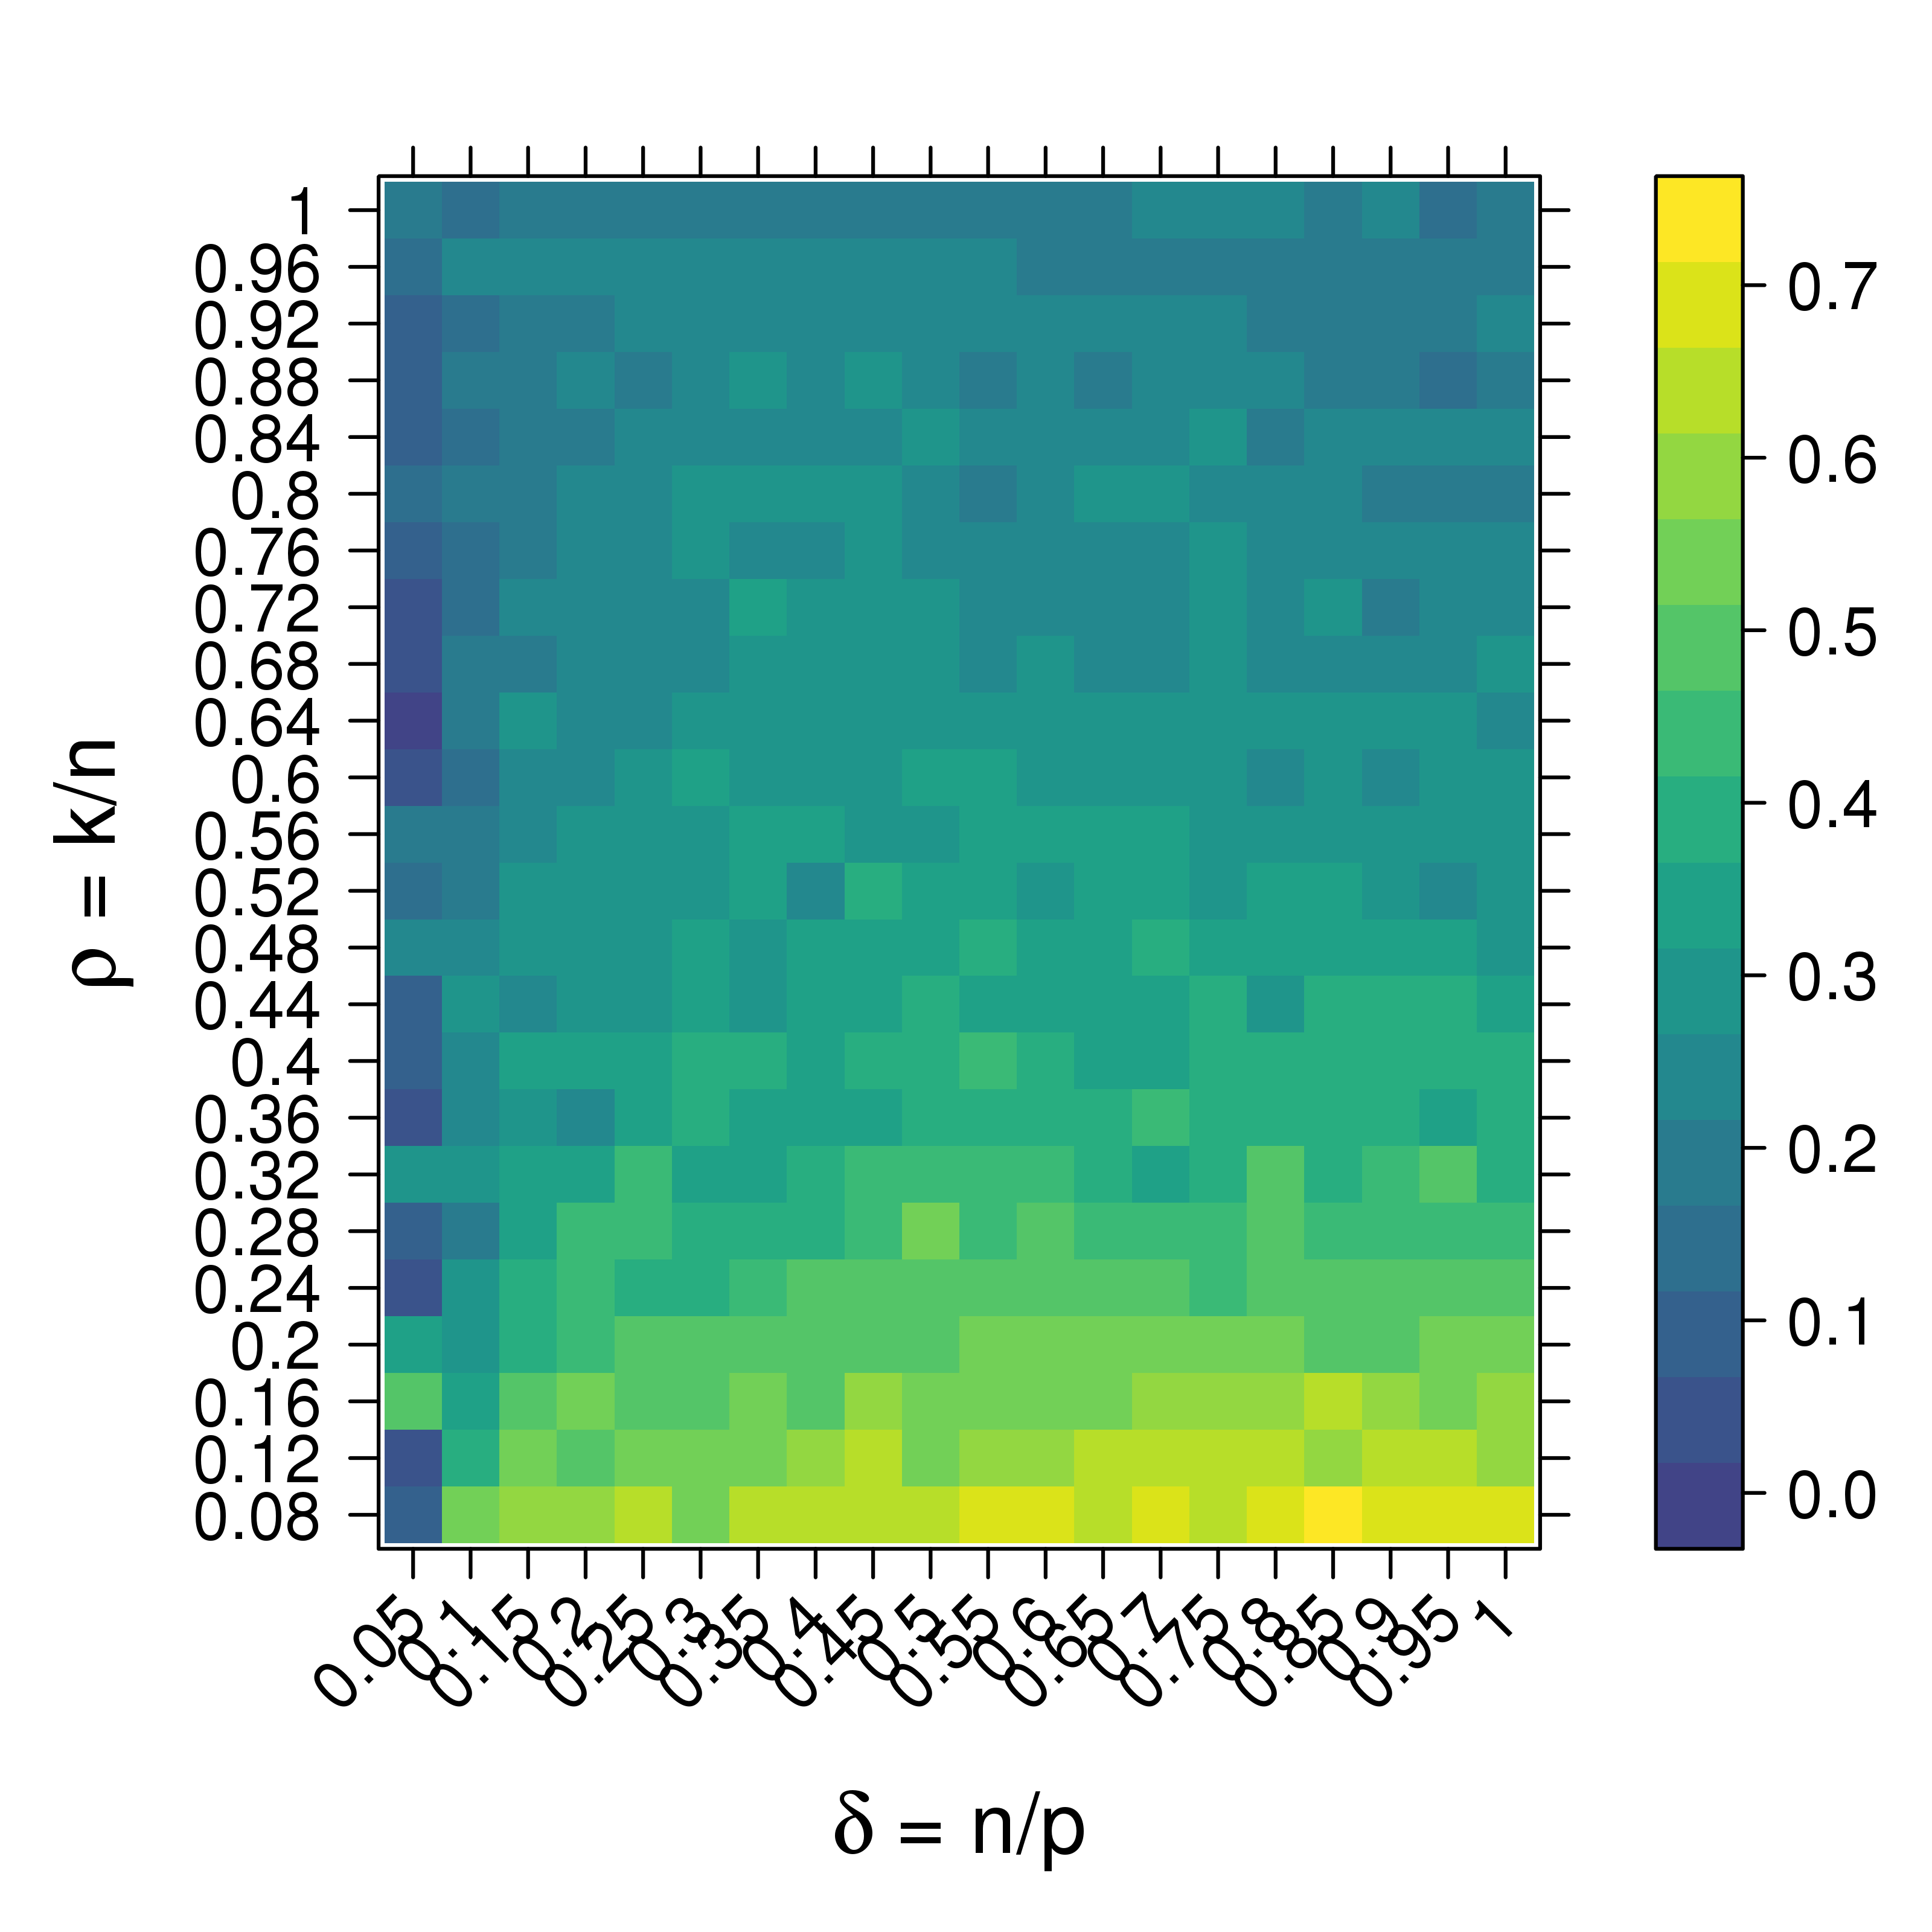
\includegraphics[totalheight=6cm]{./figs/ranger_rbo_Stodden_simulation.png}
    \caption{The RBO measure.}
    \label{figure:ranger_rbo_Stodden_simulation.png}
  \end{subfigure} 
  \caption{The  OOB error and RBO measure using a random forest.}
  \label{figure:ranger_error_and_rbo_Stodden_simulation.png}
\end{figure}

\section{The rank-biased overlap measure
  \label{section:the.Rank.biased.Overlap.measure}}

The rank-biased-overlap measure (RBO) was introduced in \cite{Webber2010}.
It provides a measure of the commonality of ranked lists with the following features:
\begin{itemize}
\item it can handle lists that are incomplete or have only some members in common;
\item weights similarity in high ranks more heavily than low;
\item it is monotonic with increasing depth of evaluation;
\item it can handle  tied ranks and rankings of different lengths.
\end{itemize}

We have included the implementation of RBO form the R package \textsc{gespeR} \cite[]{gespeR.2015},
a specialized bioinformatics package that not all users will want to install.
For a simple illustration we compare two lists:
\begin{lstlisting}
  > list1
  X1 X2 X3 X4 X5 
  5  4  3  2  1 
\end{lstlisting}
and the longer list \texttt{list2} (length 1000).
\begin{lstlisting}
  > head(list2)
  X1   X2   X3   X4   X5   X6 
  1000  999  998  997  996  995
  > rbo(list1, list2, p = 0.95)
  1
\end{lstlisting}
We then move the matching segment along one place each time i.e.
\begin{lstlisting}
  > list2[1:10]
  X6   X1   X2   X3   X4   X5  X12  X13  X14  X15 
  1000  999  998  997  996  995  994  993  992  991
  > rbo(list1, list2, p = 0.95)
  0.8
\end{lstlisting}
The $p$-value determines the witghting given to the higher rankings.
Figure \ref{figure:shift_variables.png} shows the RBO measure as the matching segement is moved along. 
% \begin{figure}[tbhp]
%  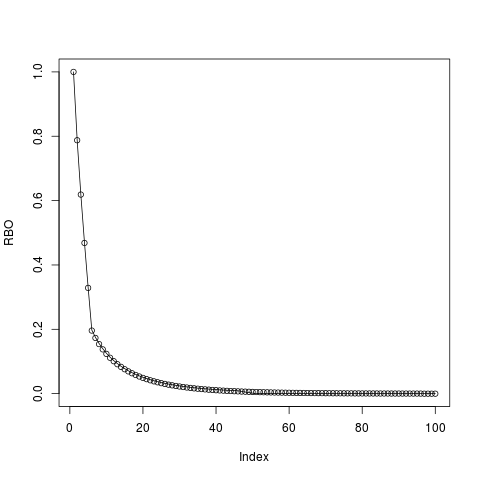
\includegraphics[totalheight=8cm]{./figs/shift_variables.png}
%  \caption{The RBO measure as \texttt{list1} is shifted along \texttt{list2}.}
%   \label{figure:shift_variables.png}
% \end{figure}

While the RBO measure is designed for integer ranks, it works and gives sensible answers for real values as well.


% \begin{figure}[tbhp]
%   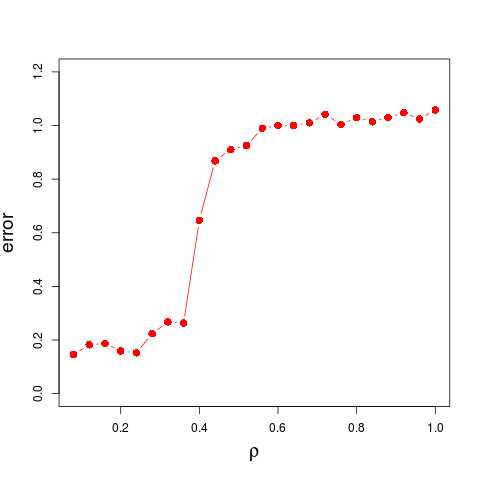
\includegraphics[totalheight=8cm]{./figs/transect.png}
%   \caption{The RBO measure as \texttt{list1} is shifted along \texttt{list2}.}
%   \label{figure:transect.png}
% \end{figure}




\begin{figure}[ht]
  \begin{minipage}[t]{0.5\linewidth}
    \centering
    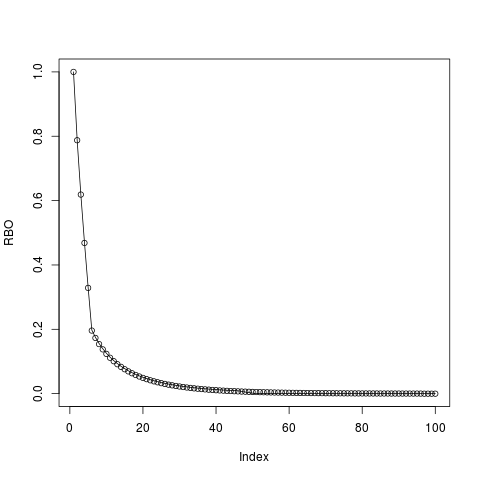
\includegraphics[width=0.8\linewidth]{./figs/shift_variables.png}
    \caption{The RBO measure as \texttt{list1} is shifted along \texttt{list2}.}
    \label{figure:shift_variables.png}
    \vspace{4ex}
  \end{minipage}%%
\hspace{4ex}
  \begin{minipage}[t]{0.5\linewidth}
    \centering
    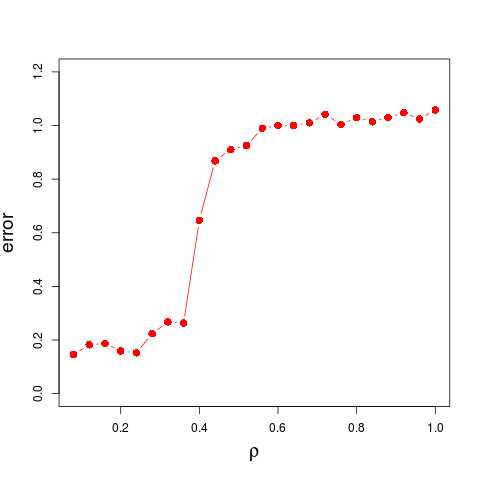
\includegraphics[width=0.8\linewidth]{./figs/transect.png}
    \caption{For $\delta=0.5$ in figure \ref{figure:error_Stodden_FDR.png}, we plot the error for values of $\rho.$} 
 \label{figure:transect.png}
    \vspace{4ex}
  \end{minipage}
\end{figure}
 


















\section{Conclusion}
We have investigated the Donoho-Tanner phase transition in a small simulation, replicating some of the work of
\cite{Donoho.and.Stodden.2006}. We have investigated the use of the RBO measure for comparing the variable importance
ranking produce by a random forest and the $\beta$ parameters in a linear model used to define the data.



\bibliography{./stepwise.bib}

\end{document}



